\documentclass[tikz]{standalone}
\usepackage{fontspec}
\renewcommand*{\familydefault}{\sfdefault}
\usepackage{standalone}
\usepackage{amssymb}
\usetikzlibrary{decorations}
\usetikzlibrary{arrows.meta, decorations.pathmorphing, decorations.pathreplacing, shapes.geometric}
\usetikzlibrary{bayesnet}

\begin{document}

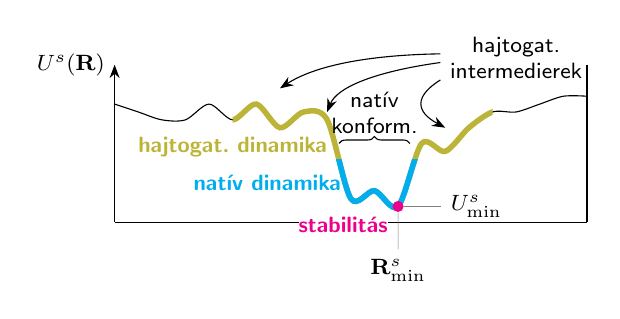
\begin{tikzpicture}[font=\footnotesize, xscale=3.0]

% axes
\draw[-Stealth] (-1,0) -- (-1,2) node[anchor=east] {\(U^s(\mathbf{R})\)} ;
\draw (1,0) -- (1,2) ;
\draw (-1,0) --
%node[anchor=north] {config.,~\(\mathbf{R}\)}
(1,0) ;

% energy landscape
\draw plot[smooth] coordinates {
(-1.0,1.5) (-0.9,1.4) (-0.8,1.3) (-0.7,1.3) (-0.6,1.5) (-0.5,1.3) (-0.4,1.5)
(-0.3,1.2) (-0.2,1.4) (-0.1,1.3) (0.0,0.3) (0.1,0.4) (0.2,0.2) (0.3,1.0) (0.4,0.9) (0.5,1.2) (0.6,1.4) (0.7,1.4) (0.8,1.5) (0.9,1.6) (1.0,1.6)
};

% hypotheses

\begin{scope}
% energy landscape
\clip (-0.5,0) rectangle (0.6,2.0);
\draw[yellow!70!black, line width=2 pt] plot[smooth] coordinates {
(-1.0,1.5) (-0.9,1.4) (-0.8,1.3) (-0.7,1.3) (-0.6,1.5) (-0.5,1.3) (-0.4,1.5)
(-0.3,1.2) (-0.2,1.4) (-0.1,1.3) (0.0,0.3) (0.1,0.4) (0.2,0.2) (0.3,1.0) (0.4,0.9) (0.5,1.2) (0.6,1.4) (0.7,1.4) (0.8,1.5) (0.9,1.6) (1.0,1.6)
};
\end{scope}

\begin{scope}
% energy landscape
\clip (-0.1,0) rectangle (0.3,0.8);
\draw[cyan, line width=2 pt] plot[smooth] coordinates {
(-1.0,1.5) (-0.9,1.4) (-0.8,1.3) (-0.7,1.3) (-0.6,1.5) (-0.5,1.3) (-0.4,1.5)
(-0.3,1.2) (-0.2,1.4) (-0.1,1.3) (0.0,0.3) (0.1,0.4) (0.2,0.2) (0.3,1.0) (0.4,0.9) (0.5,1.2) (0.6,1.4) (0.7,1.4) (0.8,1.5) (0.9,1.6) (1.0,1.6)
};
\end{scope}

\node[fill=magenta, shape=circle, inner sep=0, minimum size=4 pt,
pin=right:\(U^s_\mathrm{min}\),
pin=below:\(\mathbf{R}^s_\mathrm{min}\),
] at (0.2,0.2)
(stab) {};

% annotations
\begin{scope}[black]
\draw[decorate, decoration=brace] (-0.05,1.0) -- node[anchor=south,
align=center] (NC) {natív\\konform.} (0.25,1.0)
;
\path
(+0.7,1.7) node[align=center, anchor=south] (FI) {hajtogat.\\intermedierek}
(-0.1,1.4) coordinate (fi1)
(-0.3,1.7) coordinate (fi2)
(0.4,1.2) coordinate (fi3)
;
% arrows
\begin{scope}[-Stealth]
\draw (FI) to[bend right] (fi1) ;
\draw (FI) to[bend right] (fi2) ;
\draw (FI) to[bend right] (fi3) ;
\end{scope}
\end{scope}


% hypothesis annotations
\begin{scope}[font={\bfseries\footnotesize}]
\node[magenta, below left=5 pt, fill=white, inner sep=0] at (stab) {stabilitás};
%\node[magenta, anchor=north west, fill=white, inner sep=0] at (stab) {stability};
\node[cyan, anchor=east] at (-0.0,0.5) {natív dinamika};
\node[yellow!70!black, anchor=north] at (-0.5,1.2) {hajtogat.~dinamika};
\end{scope}

\end{tikzpicture}

\end{document}


